\section{Experimental results}

\begin{frame}{Benchmark}
    \begin{table}[]
        \begin{tabular}{|c|l|l|}
            \hline
            \textbf{Task} & \textbf{Function} & \textbf{Ideal Assisted Task} \\ \hline \hline
            $T_1$        & Sphere1            & None  \\ \hline
            $T_2$        & Sphere2            & None  \\ \hline
            $T_3$        & Sphere3            & None  \\ \hline
            $T_4$        & Weierstrass25D     & None  \\ \hline
            $T_5$        & Rosenbrock         & $T_1$  \\ \hline
            $T_6$        & Ackley             & $T_2$  \\ \hline
            $T_7$        & Weierstrass50D     & $T_3, T_4$  \\ \hline
            $T_8$        & Schwefel           & None  \\ \hline
            $T_9$        & Griewank           & $T_4$  \\ \hline
            $T_10$       & Rastrigin          & None  \\ \hline
        \end{tabular}
    \end{table}
\end{frame}

\begin{frame}{Parameter setting}
    \begin{columns}
        \begin{column}{0.48\textwidth}
            \begin{exampleblock}{MFEA}
                \begin{itemize}
                    \item Population size: 30
                    \item rmp: 0.3
                    \item sbxdi: 2
                    \item pmdi: 5
                \end{itemize}
            \end{exampleblock}
        \end{column}
        \begin{column}{0.48\textwidth}
            \begin{exampleblock}{MAB-MFEA}
                \begin{itemize}
                    \item $rmp_{min}$: $0.1$
                    \item $rmp_{max}$: $0.9$
                    \item $\alpha$: $0.01$ - discounted coefficient
                    \item $c$: $0.5$ - UCB explore/exploit trade-off coefficient
                \end{itemize}
            \end{exampleblock}
        \end{column}
    \end{columns}
    \begin{exampleblock}{MaTGA}
        \begin{itemize}
            \item $NP$:
            \item $\lambda$: $0.8$ - reward shrink rate
            \item $\rho$: $0.8$ - attenuation coefficient
            \item $\alpha$: $0.1$ - knowledge transfer rate
            \item $UR$: $0.2$ - archive update rate
            \item $AcS$: $300$ - archive size
        \end{itemize}
    \end{exampleblock}
\end{frame}

\begin{frame}{Table}
    \begin{table}[]
        \begin{tabular}{|c|c|c|c|}
            \hline
            \textbf{}      & \textbf{MFEA} & \textbf{MaTGA} & \textbf{MAB-MFEA} \\ \hline \hline
            $T_1$          & 1.32E+00      & \textbf{2.45E-04}       & 2.85E-03          \\ \hline
            $T_2$          & 1.27E+00      & 4.75E-04       & \textbf{1.15E-12}          \\ \hline
            $T_3$          & 1.17E+00      & \textbf{0}              & \textbf{6.30E-09}          \\ \hline
            $T_4$          & 3.37E+00      & \textbf{1.00E-06}       & 5.37E-04          \\ \hline
            $T_5$          & 8.15E+02      & \textbf{2.16E-02}       & 1.01E+01          \\ \hline
            $T_6$          & 1.99E+01      & 3.61E-03       & \textbf{1.05E-07}          \\ \hline
            $T_7$          & 1.05E+01      & \textbf{5.57E-04}       & 1.52E-03          \\ \hline
            $T_8$          & 2.34E+03      & \textbf{3.40E-02 }      & 9.21E+02          \\ \hline
            $T_9$          & 4.11E-02      & 4.52E-03       & \textbf{4.50E-03}          \\ \hline
            $T_10$         & 1.55E+01      & 1.57E+01       & \textbf{7.77E+00}          \\ \hline
        \end{tabular}
        \caption{The performance of 3 algorithms for 30 independent runs}
    \end{table}
\end{frame}

\begin{frame}{Analysis}
    \begin{figure}
        \begin{subfigure}[b]{0.27\linewidth}
            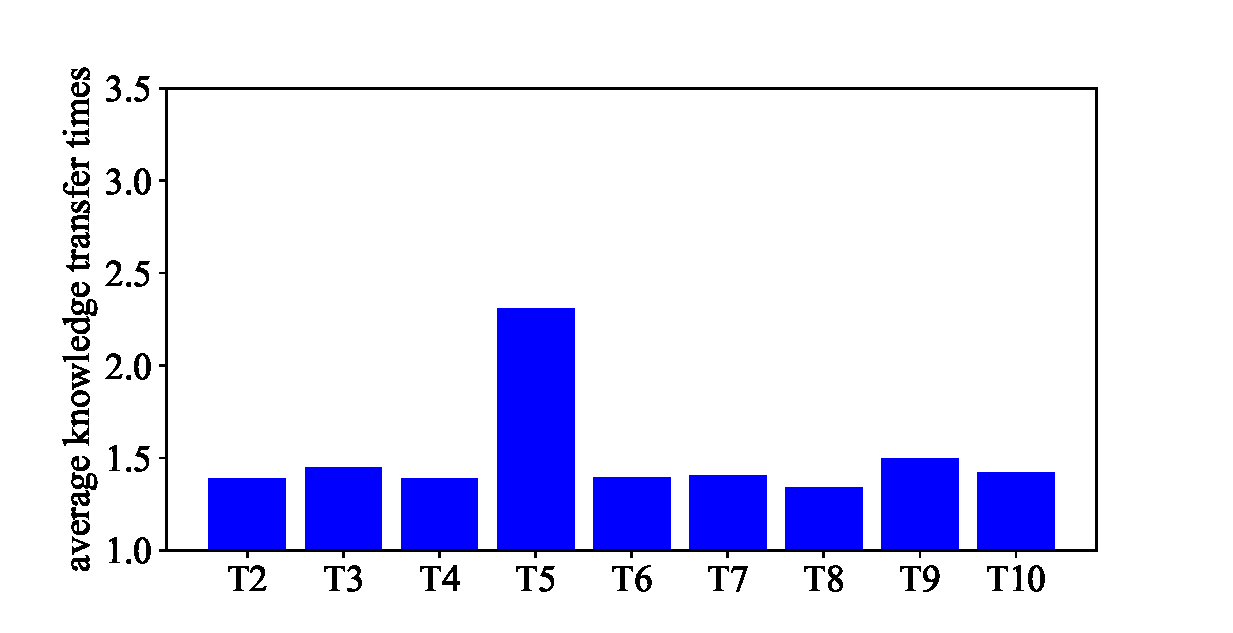
\includegraphics[width=\textwidth]{figure/count/1.eps}
            \caption{Task 1}
        \end{subfigure}
        \begin{subfigure}[b]{0.27\linewidth}
            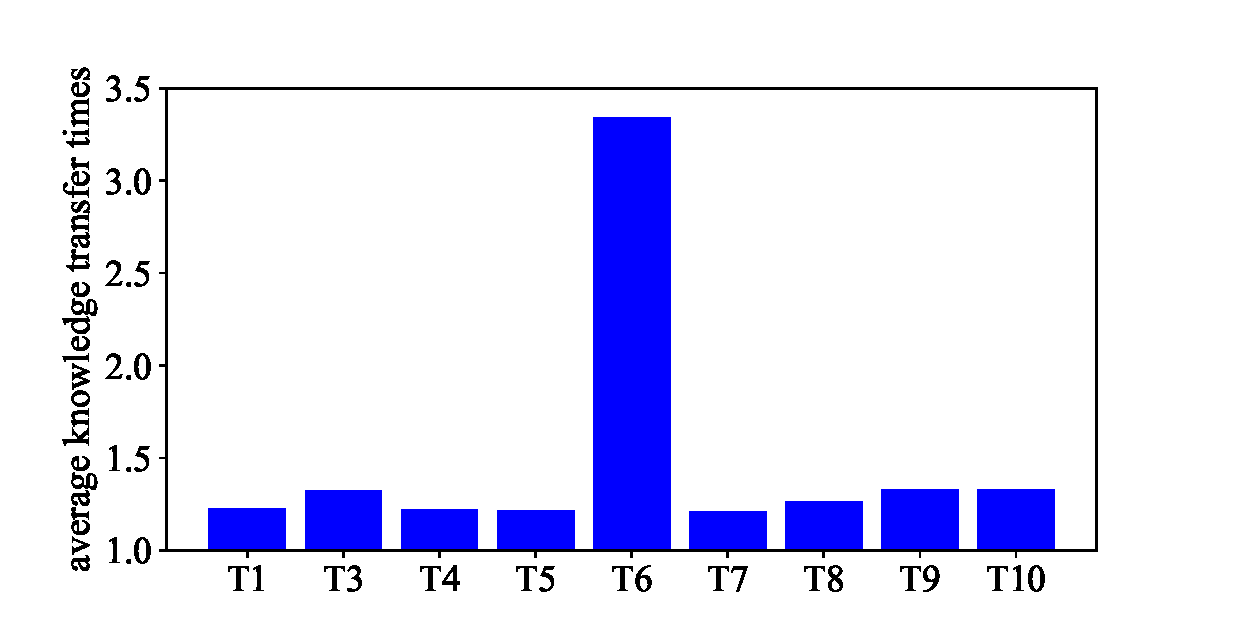
\includegraphics[width=\textwidth]{figure/count/2.eps}
            \caption{Task 2}
        \end{subfigure}
        \begin{subfigure}[b]{0.27\linewidth}
            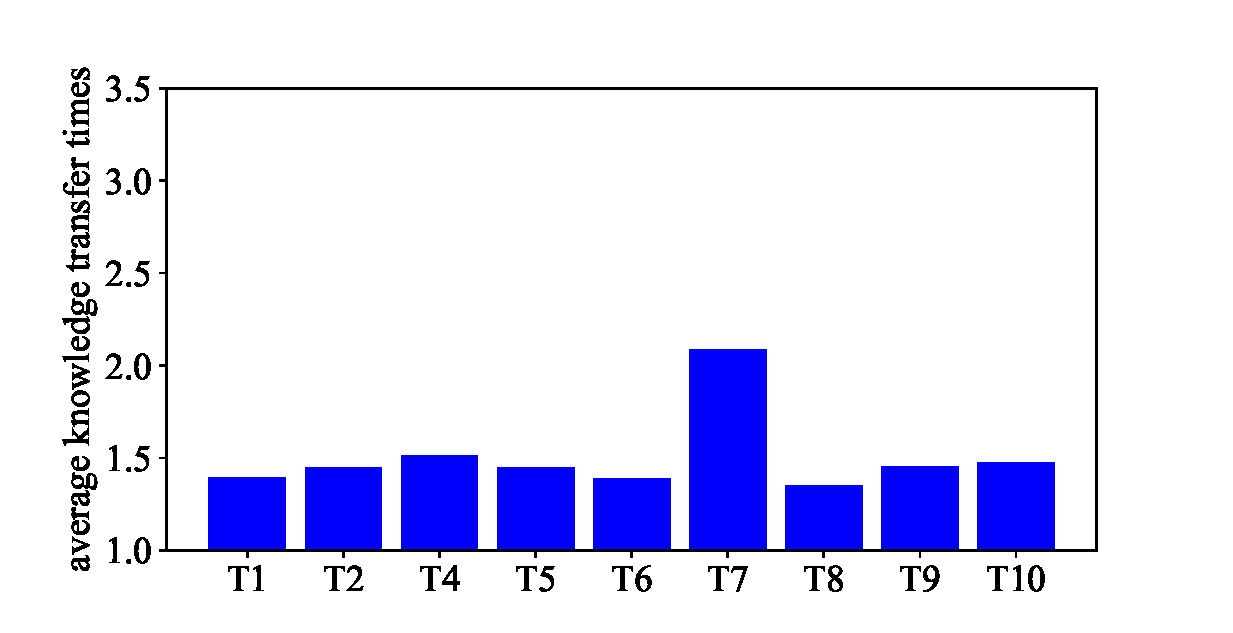
\includegraphics[width=\textwidth]{figure/count/3.eps}
            \caption{Task 3}
        \end{subfigure}

        \begin{subfigure}[b]{0.27\linewidth}
            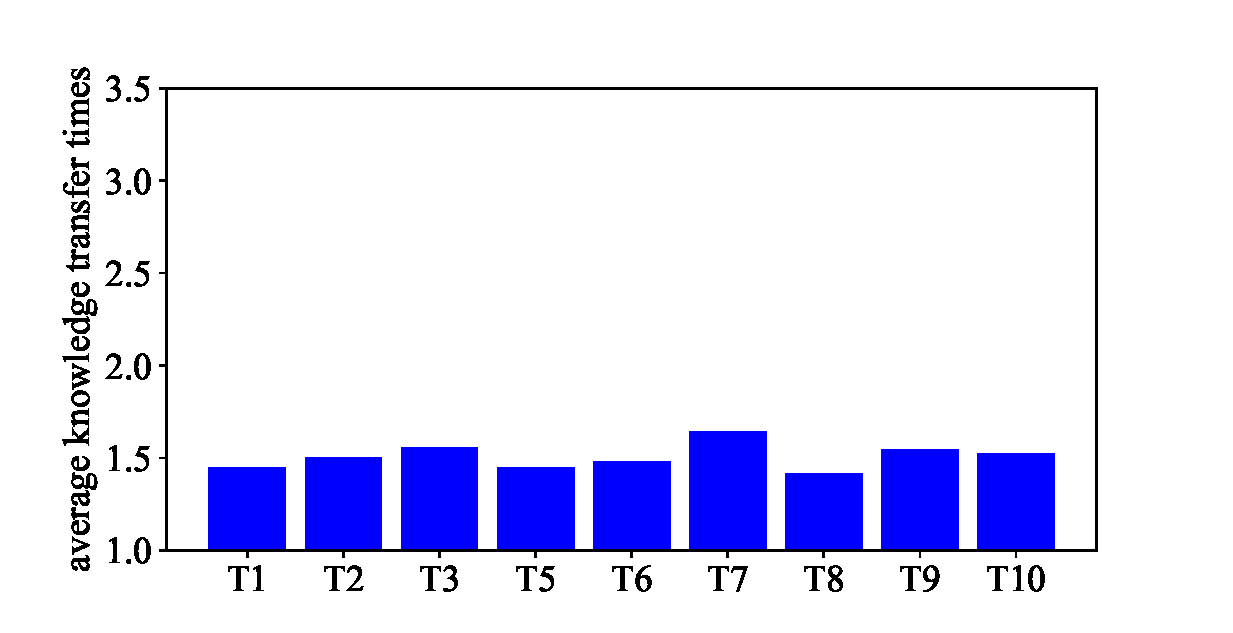
\includegraphics[width=\textwidth]{figure/count/4.eps}
            \caption{Task 4}
        \end{subfigure}
        \begin{subfigure}[b]{0.27\linewidth}
            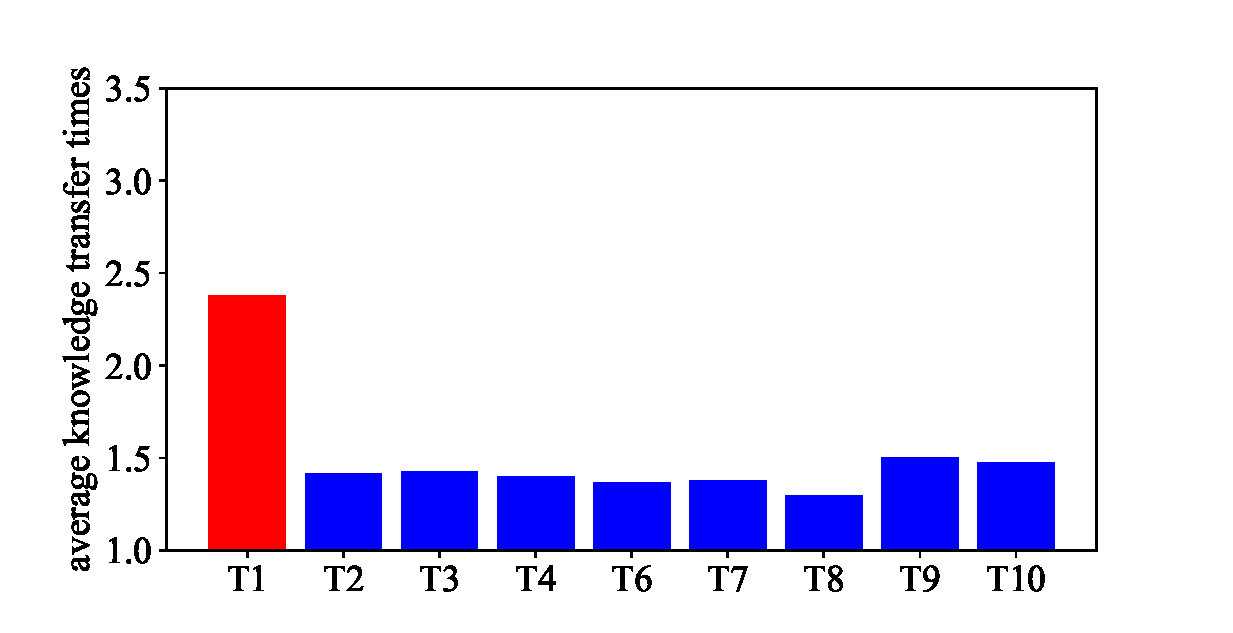
\includegraphics[width=\textwidth]{figure/count/5.eps}
            \caption{Task 5}
        \end{subfigure}
        \begin{subfigure}[b]{0.27\linewidth}
            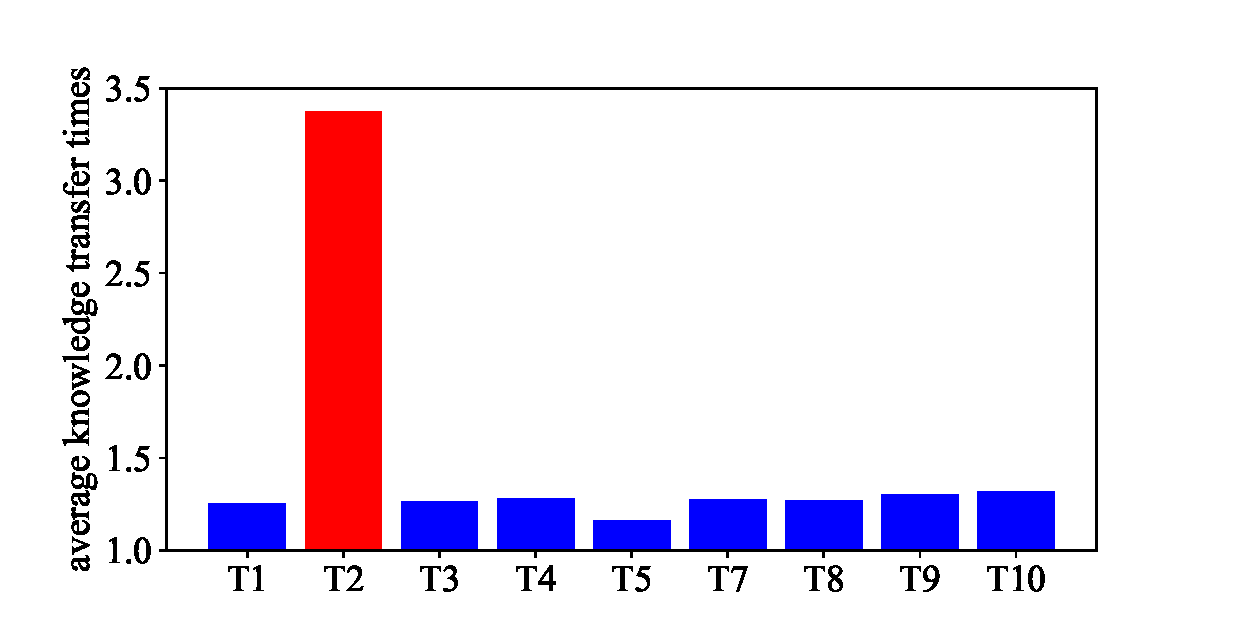
\includegraphics[width=\textwidth]{figure/count/6.eps}
            \caption{Task 6}
        \end{subfigure}

        \begin{subfigure}[b]{0.27\linewidth}
            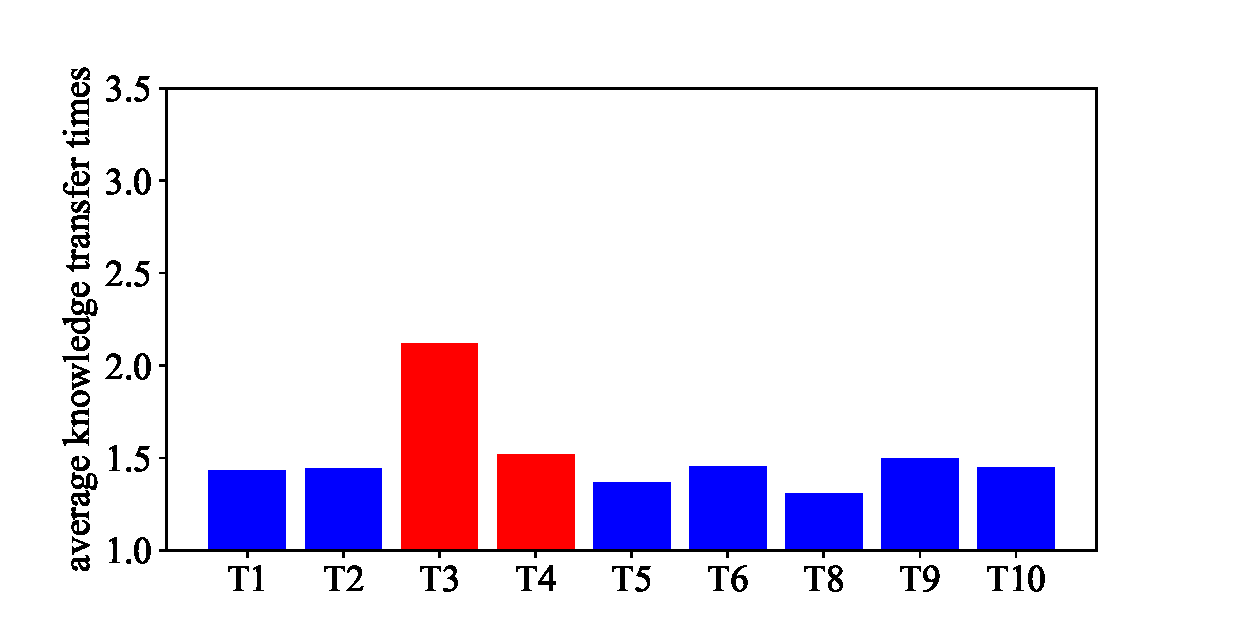
\includegraphics[width=\textwidth]{figure/count/7.eps}
            \caption{Task 7}
        \end{subfigure}
        \begin{subfigure}[b]{0.27\linewidth}
            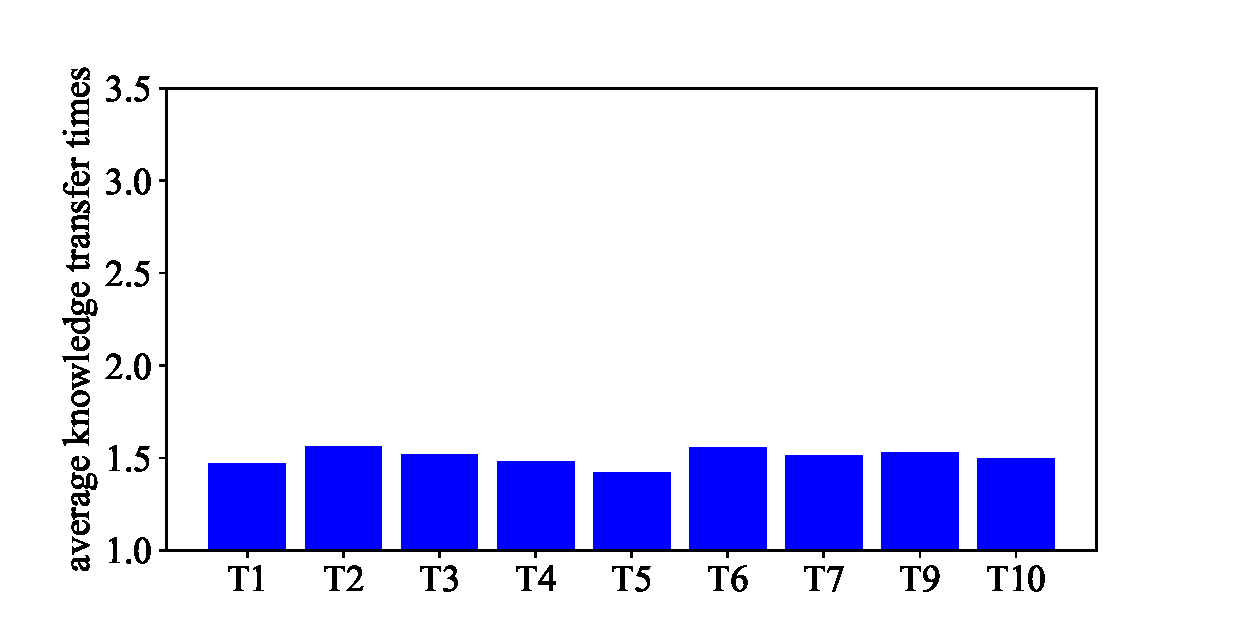
\includegraphics[width=\textwidth]{figure/count/8.eps}
            \caption{Task 8}
        \end{subfigure}
        \begin{subfigure}[b]{0.27\linewidth}
            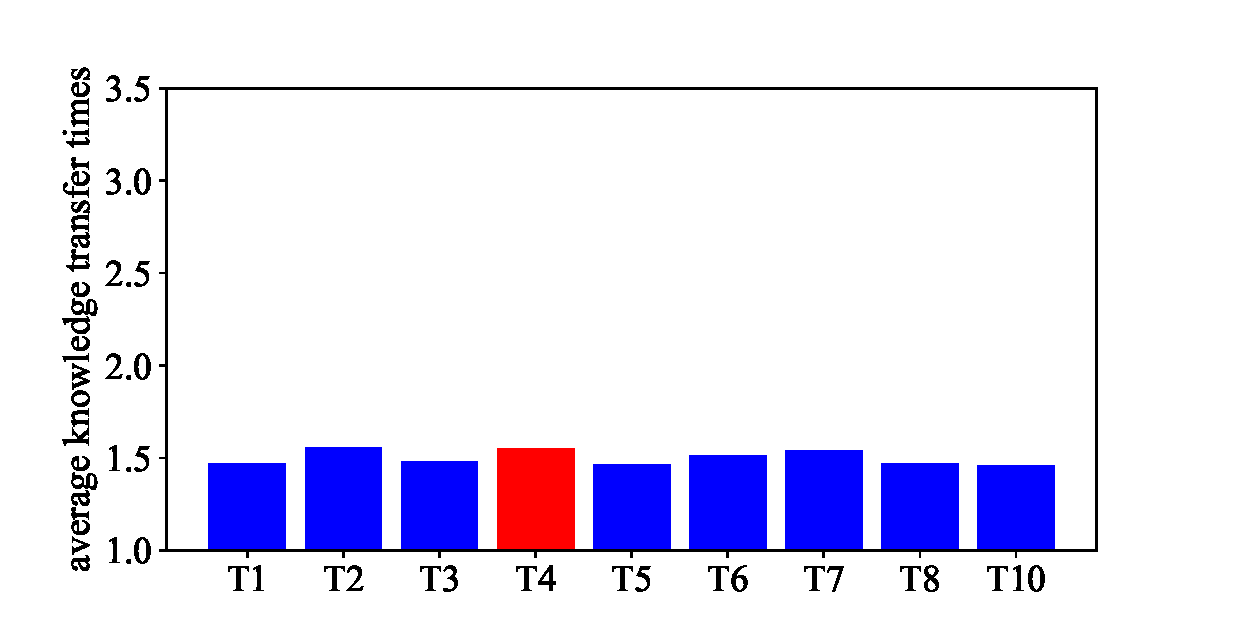
\includegraphics[width=\textwidth]{figure/count/9.eps}
            \caption{Task 9}
        \end{subfigure}

        \caption{The average times of choosing knowledge transfer target, the assisted task is highlighted in red}
    \end{figure}
\end{frame}

\begin{frame}{Analysis}
    \begin{figure}
        \begin{subfigure}[b]{0.32\linewidth}
            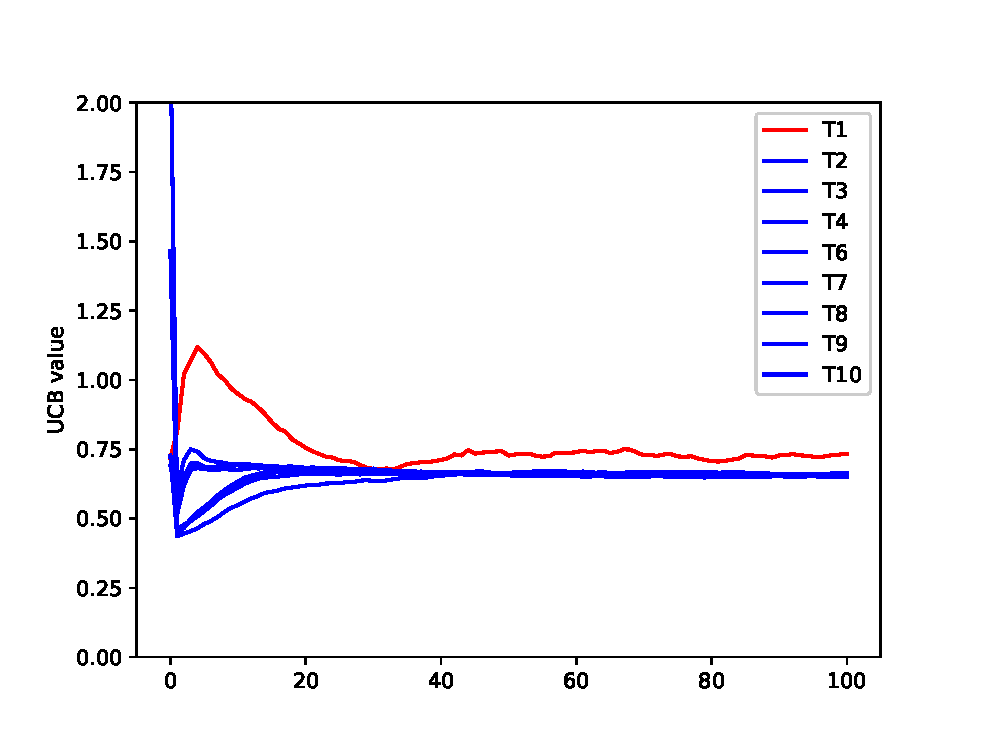
\includegraphics[width=\linewidth]{figure/ucb/5.eps}
            \caption{Task 5}
        \end{subfigure}
        \begin{subfigure}[b]{0.32\linewidth}
            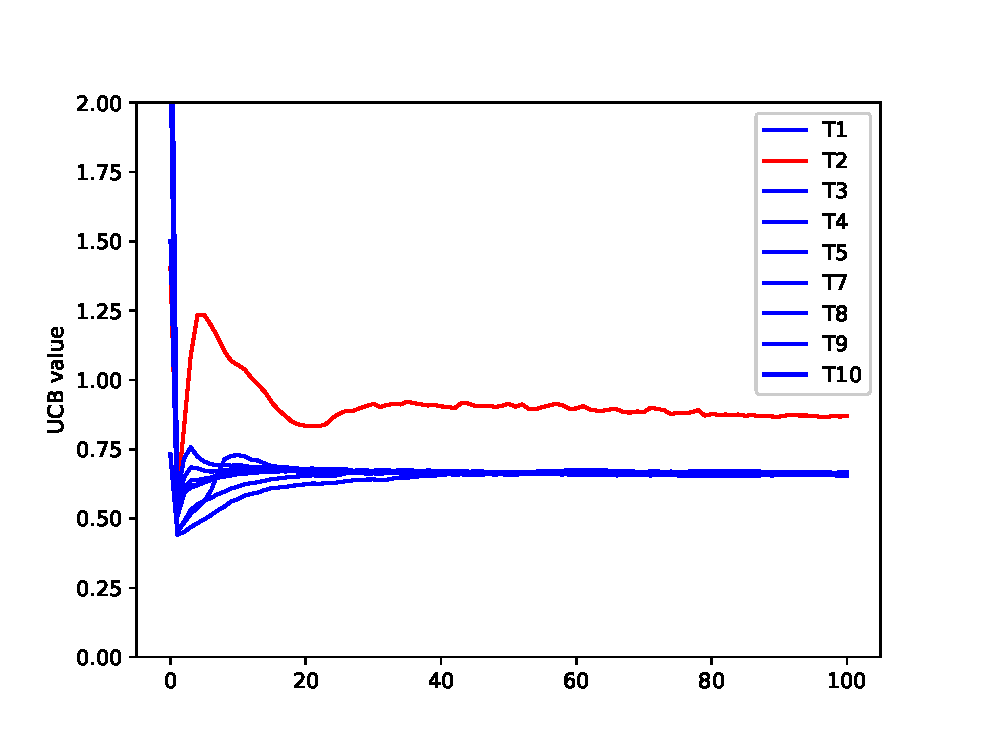
\includegraphics[width=\linewidth]{figure/ucb/6.eps}
            \caption{Task 6}
        \end{subfigure}
        \begin{subfigure}[b]{0.32\linewidth}
            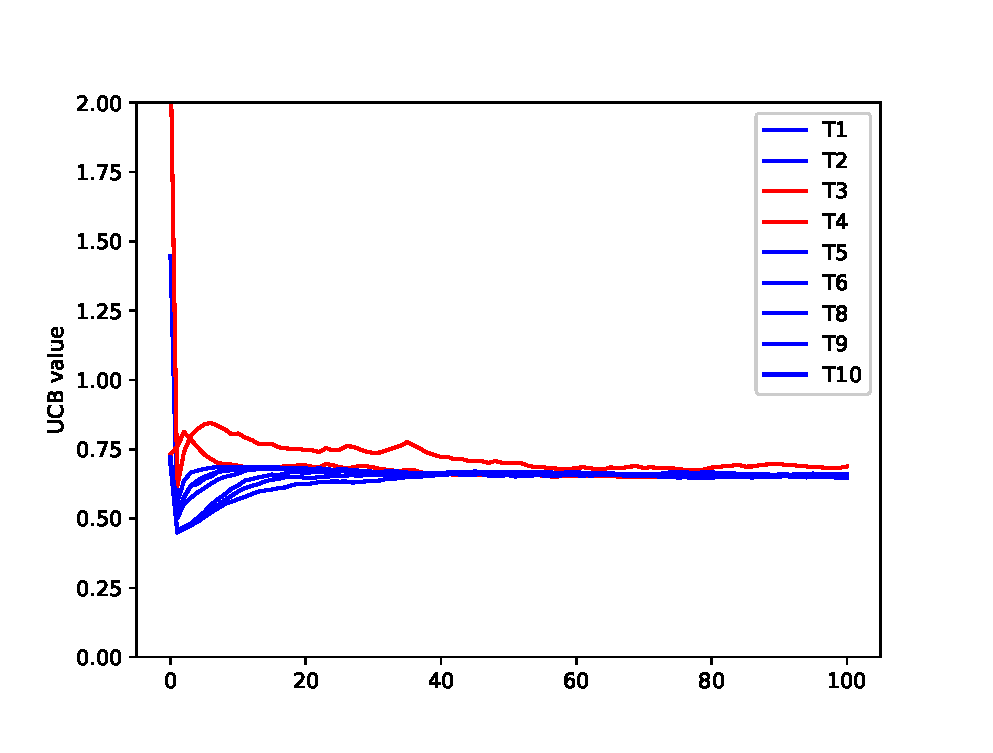
\includegraphics[width=\linewidth]{figure/ucb/7.eps}
            \caption{Task 7}
        \end{subfigure}
        \caption{The UCB function value for choosing knowledge transfer target, the assisted task is highlighted in red}
    \end{figure}
\end{frame}